\section{評価実験} \label{sec:evaluation}


ソフトウェア若化を行う VampOS のプロトタイプを Unikraft 0.8.0 に実装し,予備実験を行った.
実験には,
Intel Xeon E5-2430 v2 (6 コア,2.5 GHz)と 16 GB の RAM を搭載する
PowerEdge T320 をハイパースレッディングを無効にして使用した.
本実験では,
ソフトウェア若化に関する基礎的な疑問である
VampOS に伴うオーバヘッドと
実アプリケーションおける VampOS の効果を確認することを目的とする.

\subsection{マイクロベンチマーク}

\begin{figure}[!t]
    \centering
    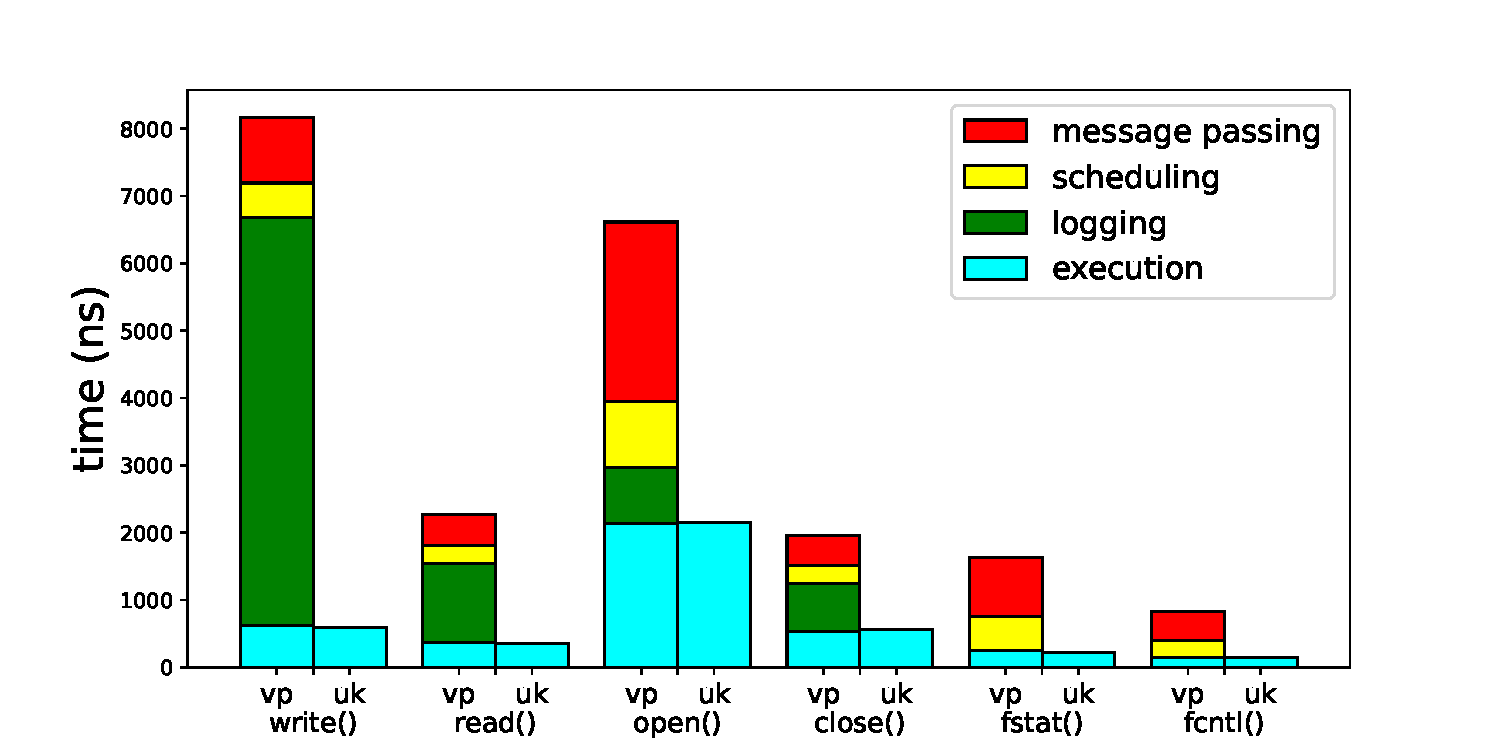
\includegraphics[width=\linewidth]{img/syscall-time.pdf}
    \caption{システムコールのオーバヘッド}
    \label{fig:func-time}
\end{figure}

VampOS によって生じるランタイムオーバヘッドを確認するために,
プロトタイプとデフォルトの Unikraft におけるシステムコールの実行時間を計測した.
特に,
\textbf{write()},\textbf{read()},\textbf{open()},\textbf{close()},\textbf{fstat()},\textbf{fcntl()} の 6 つのシステムコールの実行時間を計測した.
\textbf{write()},\textbf{read()} においては,
それぞれ,1 バイトのファイルに対して命令を発行している.
\textbf{open()},\textbf{close()} においては,
ファイルに対してただファイルディスクリプタを作成し,解放するという操作のみを行う.
\textbf{fstat()}では,ファイルの状態を取得し,
\textbf{fcntl()}では,ファイルディスクリプタのフラグを取得する.
\textbf{fcntl()}を除くこれらのシステムコール実行時には,VFS と RAMFS コンポーネント間のインタラクションが発生するのに対し,
\textbf{fcntl()}では,VFS コンポーネントのみを使用する.


実験の結果を
図\ref{fig:func-time}に示す,
図の横軸はシステムコールの種類を,
縦軸はその実行時間を表している.
図より,プロトタイプは最大で 13.60 倍のランタイムオーバヘッドを生じている.
このオーバヘッドは,デフォルトの Unikraft にはない \sysname におけるコンポーネントごとのスレッドのスケジューリングや
再起動後の動作状態を復元するための関数呼び出しのロギング,コンポーネントスレッド間のメッセージパッシング方式でのデータの受け渡し
によるものである.
また,
ランタイムオーバヘッドは元のシステムコールの実行時間が短いほど,
その倍率が大きくなる.
実際に,デフォルトの Unikraft と比較して,
\sysname の \textbf{read()} の実行時間が 6.38 倍であるのに対し,
\textbf{open()} の実行時間は 3.06 倍である.

\sysname の追加の仕事にかかる時間は,
システムコールの種類に依存する.
\textbf{write()} のロギングにかかる時間は,
他のシステムコールよりも復元のためにより多くのデータを記録するため,最も長くなる.
一方で,
\textbf{open()} のデータ受け渡しにかかる時間が最も長いのは,
VFS と RAMFS コンポーネントが互いに実装された関数を呼び合い,
その実行のために追加のスレッドの生成されるためである.


\subsection{マクロベンチマーク}

\begin{figure}[!t]
    \centering
    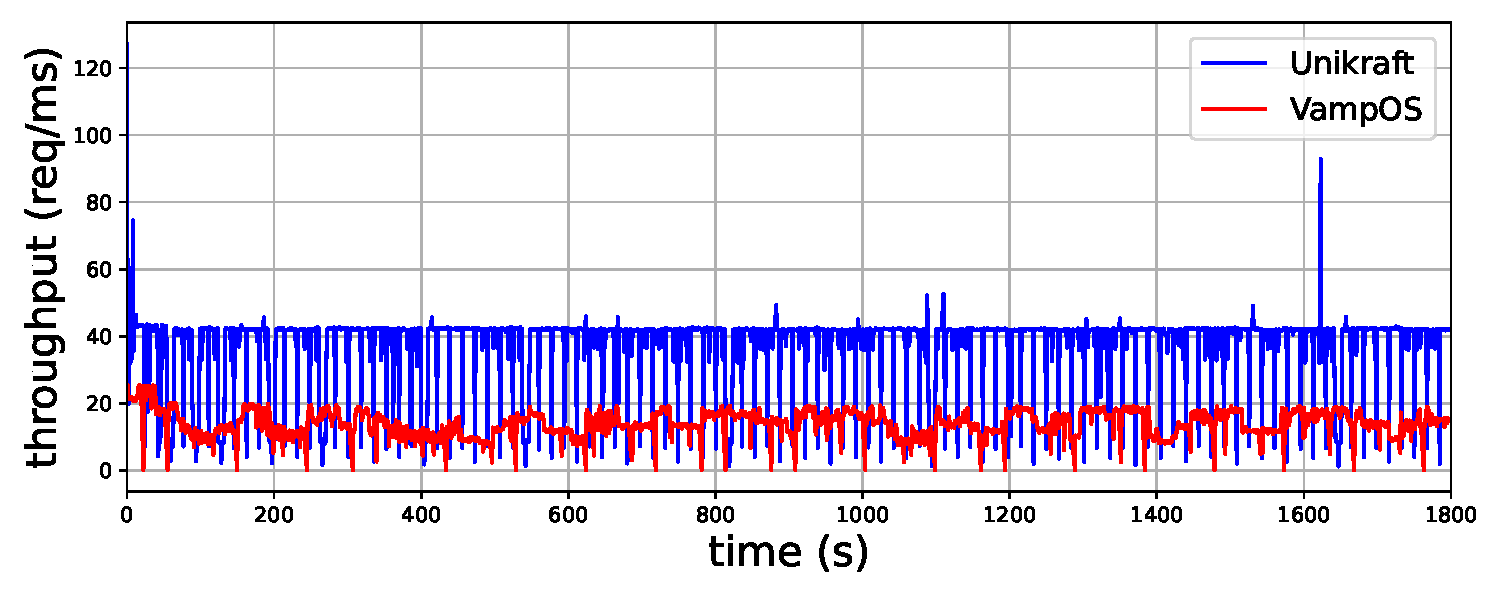
\includegraphics[width=\linewidth]{img/SQLite-perf.pdf}
    \caption{SQLite のスループット}
    \label{fig:sqlite-perf}
\end{figure}

\begin{figure}[!t]
    \centering
    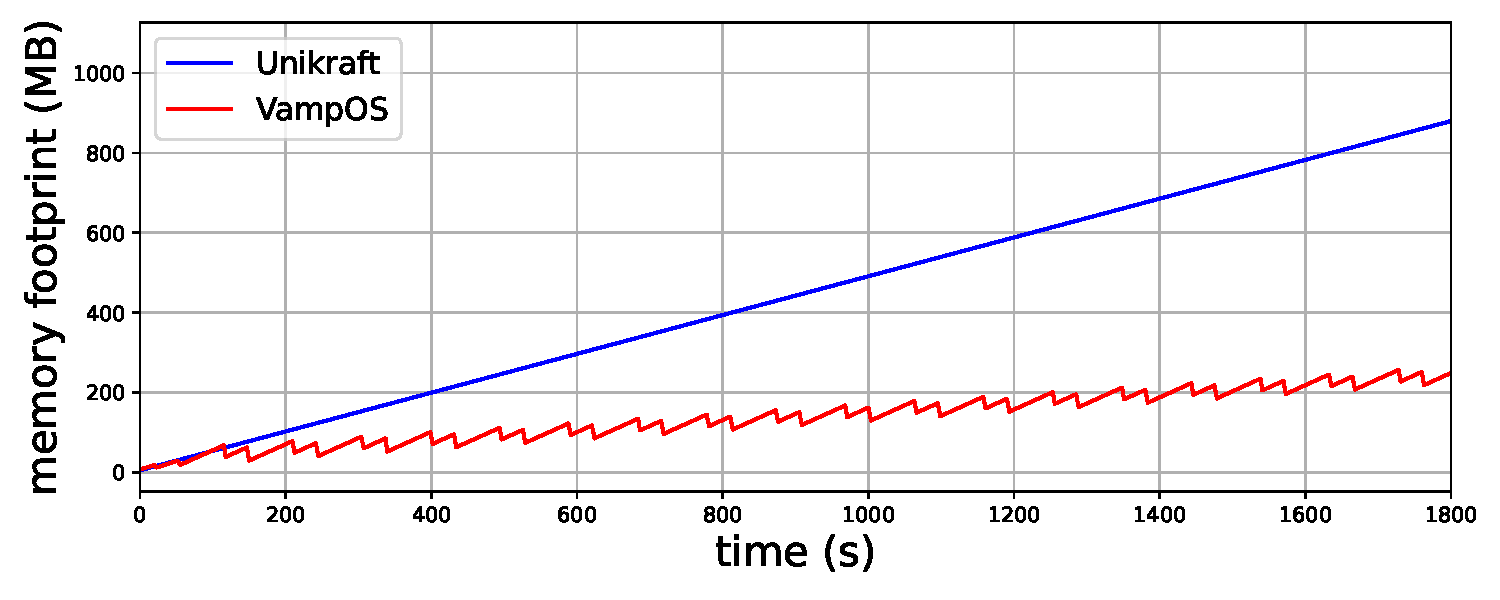
\includegraphics[width=\linewidth]{img/SQLite-mem.pdf}
    \caption{SQLite のメモリ消費量}
    \label{fig:sqlite-mem}
\end{figure}

実アプリケーションに対する \sysname の有効性を確認するために,
\sysname で SQLite を実行した.
SQLite は,汎用的なリレーショナル・データベース管理システム(RDBMS)であり,
Unikraft がサポートするアプリケーションの一つである.
本実験では,意図的にメモリリークのバグを挿入した \sysname で SQLite を起動し,
SELECT リクエストのスループットとメモリ消費量を計測する.
\sysname によるコンポーネントの若返りを行いながら,
SQLite を 30 分間動作させ続ける.
\sysname は,
VFS,RAMFS,スケジューラといった状態を持つ SQLite の Unikernel コンポーネントの若返りをラウンドロビン方式で行う.
\sysname は 30 秒ごとに一つずつコンポーネントの若返りを行う.
基準として,再起動を行わないデフォルトの Unikraft のスループットとメモリ消費量を計測する.
Unikraft の再起動は,RAM ファイルシステム上のデータベースの削除を伴い,
再起動を通して動作を継続できないため,
SQLite の若返りに使用することはできない.

図\ref{fig:sqlite-perf},\ref{fig:sqlite-mem} は,それぞれ,実験における SQLite のスループットとメモリ消費量を示している.
図\ref{fig:sqlite-perf} から,\sysname の若返りのための頻繁な再起動に対する長いダウンタイムを生じないことが分かる.
また,\sysname 上の SQLite のスループットは,デフォルトの Unikraft と同様に 30 秒ごとのコンポーネント単位の若返りをしながらも安定している.
しかし,前述したランタイムオーバヘッドにより,プロトタイプでのスループットがデフォルトの Unikraft の 半分程度になってしまう.
次の章では,実行時オーバーヘッドを軽減するために最適化が必要であることを述べる.


図\ref{fig:sqlite-mem} は,\sysname のプロトタイプがメモリリークを緩和していることを示している.
デフォルトの Unikraft のメモリ消費量は,
挿入したメモリリークのバグの影響で
線形に増加している.
一方,\sysname のログサイズが時間とともに増加するため,
プロトタイプのメモリ消費量は徐々に増加する.
\sysname のメモリオーバヘッドは,デフォルトの Unikraft のメモリ増加量よりも遥かに少ない.
今後,復元に不要なログを定期的に削除するなどのログのメモリ消費量を削減する仕組みを検討することが必要になる.
